\documentclass[a4paper, 11pt]{article}

\usepackage{graphicx}


\usepackage{wrapfig}
\usepackage{lipsum}

\usepackage[utf8]{inputenc}

\usepackage{mathpazo} % Use the Palatino font
\usepackage[T1]{fontenc} % Required for accented characters
\linespread{1.05} % Change line spacing here, Palatino benefits from a slight increase by default

\usepackage{float}
\usepackage{hyperref}
\hypersetup{
	colorlinks=true, 		% Aktivieren von farbigen Links im Dokument
	linkcolor=blue, 	% Farbe festlegen
	urlcolor=blue,
	linktocpage=true, 		% Nicht der Text sondern die Seitenzahlen in Verzeichnissen klickbar
	bookmarksnumbered=true 	% Überschriftsnummerierung im PDF Inhalt anzeigen.
}
\usepackage[ngerman]{babel}
\usepackage{tabularx}
\usepackage[table,xcdraw]{xcolor}
\usepackage{listings}
\usepackage{enumitem}

\makeatletter

\renewcommand{\maketitle}{ % Customize the title - do not edit title and author name here, see the TITLE block below
\begin{flushright} % Right align
{\LARGE\@title} % Increase the font size of the title

\vspace{10pt} % Some vertical space between the title and author name

{\large\@author} % Author name
\\\@date % Date

\vspace{20pt} % Some vertical space between the author block and abstract
\end{flushright}
}

\title{\textbf{Technische Dokumentation des Gesamtprojekts}} 


\date{\today} % Date
\author{Matthis Gördel}

\begin{document}
\renewcommand{\@listI}{\itemsep=0pt} % Reduce the space between items in the itemize and enumerate environments and the bibliography


\maketitle % Print the title section

\begin{abstract}
    Das MdWI-Projekt der Semester fünf und sechs wird als agiles
    Softwareprojekt durchgeführt. Für die Umsetzung wurde die Entscheidung
    getroffen, den Kurs in drei Teams aufzuteilen: \emph{Marketing},
    \emph{Frontend} und \emph{Backend}. Hier wird die Motivation hinter dieser
    Trennung, verbunden mit der technischen Architektur, beschrieben.
\end{abstract}

\section{Ausgangssituation}

Zu Beginn gab für die Umsetzung des Projekts zwei zentrale Fragen:

\begin{itemize}
    \item Wie soll die technische Architektur aussehen?
    \item Wie organisieren wir uns als Kurs?
\end{itemize}

Als Rahmenparameter war gegeben, dass das Projekt per Scrum organisiert werden
soll. Dies bringt einige Implikationen für die Entwicklung mit sich, da Scrum
interdisziplinäre Entwicklerteams fordert, im Gegensatz zu zum Beispiel einer
Aufteilung in Entwicklungs-, Datenbank-, und Test-Team.

Scrum fordert außerdem Teams von rund sieben Mitarbeitern. Den Kurs in drei
Teams aufzuteilen, schien deshalb sinnvoll. Daraus ergab sich die Frage nach
einer geeigneten technischen Architektur, bei der mehrere Entwicklerteams
parallel an einem Produkt arbeiten können. Da eine Webapplikation entwickelt
werden sollte, wurden zwei Optionen gesehen:

\begin{itemize}
    \item Die Umsetzung als Monolith.
    \item Die Umsetzung als Single-Page-Anwendung mit getrenntem Front- und
        Backend. 
\end{itemize}

Eine Umsetzung als \emph{monolithische} Applikation hätte zum Beispiel so
aussehen können, dass zum Beispiel mit PHP und HTML oder einem Webframework mit
HTML-Template-Engine von mehreren Teams eine einzige Applikation entwickelt
wird.

Die Alternative wäre, eine \emph{Single-Page-Anwendung} mit Webservice-Backend
zu entwickeln. Hier entwickelt ein Team eine Webanwendung, welche vom Endnutzer
als ein einziges HTML-Dokument heruntergeladen wird, welches daraufhin
anzuzeigende Inhalte dynamisch von einem Backend-Server abfragt, der von einem
anderen Team entwickelt wird. Hier ist die Website eine art \emph{Fat-Client},
da die Website, die der Nutzer herunterlädt, viel mehr Logik enthält als die
verschiedenen Webseiten, die eine monolitische Applikation generiert.

\begin{table}
    \centering
    \begin{tabularx}{\textwidth}[htbp]{|l|X|X|}
        \hline
        \rowcolor[HTML]{E0E0E0}
        & \textbf{Monolith} & \textbf{Single-Page-Application}
        \\ \hline
        Vorteile & 
        \begin{itemize}[noitemsep,topsep=0pt,parsep=0pt,partopsep=0pt]
            \item Alle arbeiten mit einer Sprache, einem Framework
            \item Flexiblerer Einsatz der Entwickler
        \end{itemize}
        &
        \begin{itemize}[noitemsep,topsep=0pt,parsep=0pt,partopsep=0pt]
            \item Entkopplung in zwei Anwendungen: Frontend und Backend 
            \item Mehr, an dem parallel gearbeitet werden kann
        \end{itemize}
        \\ \hline
        Nachteile   &
        \begin{itemize}[noitemsep,topsep=0pt,parsep=0pt,partopsep=0pt]
            \item Eventuell komplexer Spaghetti-Code
            \item Schwierig, > 10 Entwickler parallel zu beschäftigen
        \end{itemize}
        &
        \begin{itemize}[noitemsep,topsep=0pt,parsep=0pt,partopsep=0pt]
            \item Herausforderung der Absprache zw. Front- und Backend
            \item Abhängigkeiten
        \end{itemize}
        \\ \hline
    \end{tabularx}
    \caption{Vor- und Nachteile der techn. Ansätze}
    \label{tab:pro_contra}
\end{table}

Es wurde die Ansätze abgewogen (vgl. Tabelle \ref{tab:pro_contra}) und sich
gegen den monolitischen Ansatz entschieden. Daraus resultierte nun endgültig
die Teilung in \emph{Frontend} und \emph{Backend} (und \emph{Marketing}).

\section{Single-Page-Anwendung, Frontend, Backend}

\begin{figure}[htpb]
    \centering
    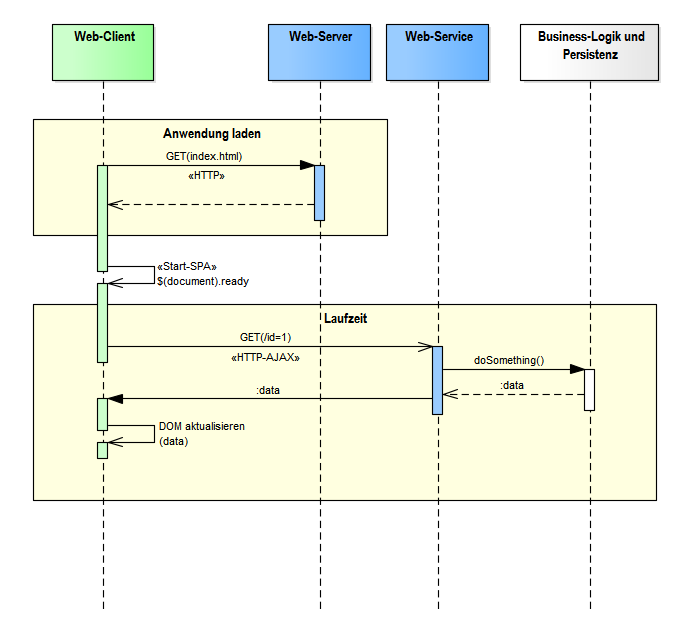
\includegraphics[width=10cm]{images/SPA_Start.png}
    \caption{Skizzierung des Ablaufs einer Single-Page-Webanwendung}
    \label{fig:spa_start}
\end{figure}

Abildung \ref{fig:spa_start} zeigt die Funktionsweise einer
Single-Page-Anwendung. Im ersten hervorgehobenen Rechteck wird das Laden der
Anwendung darstegellt. Ein Anwender ruft zum Beispiel die Webseite der
Projekt-Anwendung auf. Sein Browser schickt dann eine GET-Request nach der
\texttt{index.html}, der zentralen HTML-Seite. Diese wird vom Webserver
beantwortet. Nun hat der Anwender die Anwendung in den Speicher seines Browsers
geladen. 

Wenn nun der Anwender zum Beispiel seine Mitgliedsdaten sehen möchte, klickt er
im Browser auf den entsprechenden Link. Es wird jedoch keine neue HTML-Seite
aufgerufen und heruntergeladen, sondern die Webanwendung schickt stattdessen
eine Anfrage an einen Webservice, das \emph{Backend}. Dieser prüft dann zum
Beispiel, ob die Anfrage berechtigt ist und greift auf die Datenbank zu um die
angeforderten Daten zu lesen.

Daraufhin schickt er die Daten an die Webanwendung im Browser des Nutzers
zurück, welche dann entscheidet, wie diese Daten dargestellt werden sollen und
dann das HTML, also den Aufbau der Seite, dynamisch verändert.

Es ist also ein bisschen so, als ob der Nutzer beim Öffnen der Seite ein
Programm herunterlädt und mit diesem interagiert. Das Programm wiederum greift
auf einen Server zu, schickt und holt Daten. Schließt der Anwender das
Browserfenster löscht/deinstalliert er das Programm sozusagen.

Die Kommunikation zwischen der Anwendung im Browser und dem Webservice erfolgt
über eine Webschnittstelle. Die Anwendung ruft also Webseiten auf, wobei diese
aber nicht für Menschen gedacht sind, sondern einfach nur Daten in einer
relativ rohen Form enthalten.

\section{Die API-Spec}

Im Projekt erfolgt die Definition und Dokumentation dieser Web-Schnittstelle
über die sogenannte \href{https://wwi16ama.feste-ip.net/swagger/}{API-Spec}.
Hier werden die möglichen Routen, die die Frontend-Anwendung aufrufen kann,
definiert. Genauso werden die eventuell notwendigen Parameter der Anfragen und
die möglichen Ergebnisse beschrieben.

\begin{figure}[htpb]
    \centering
    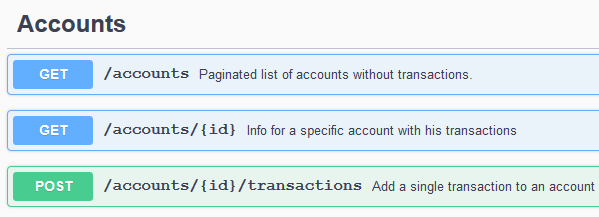
\includegraphics{images/api_spec_example_short.png}
    \caption{Übersicht der möglichen Routen zu Accounts}
    \label{fig:api_spec_accs}
\end{figure}

Abbildung \ref{fig:api_spec_accs} zeigt einen Auszug aus der API-Speck. Hier
wurden unter der Überschrift \emph{Accounts} drei verschiedene Routen
zugegriffen, auf die jeweils mit verschiedenen HTTP-Methoden zugegriffen wird.
Rechts steht eine Beschreibung, was mit dem Aufruf geschieht. Dies ist jedoch nur die Kompakt-Ansicht, die sich expandieren lässt.

Ein Ausschnitt der expandierten Darstellung ist in Abbildung
\ref{fig:api_spec_post} zu sehen. Hier wird beschrieben, welche Parameter für
die Anfrage notwendig sind. Das ist zum einen ein Parameter in der URL des
Aufrufs, um anderen muss beim \texttt{POST} eine Art Anhang mitgeschickt
werden, nämlich das Objekt im \emph{Request Body}, welches den Betrag und den
Transaktionstyp enthält.

\begin{figure}[htpb]
    \centering
    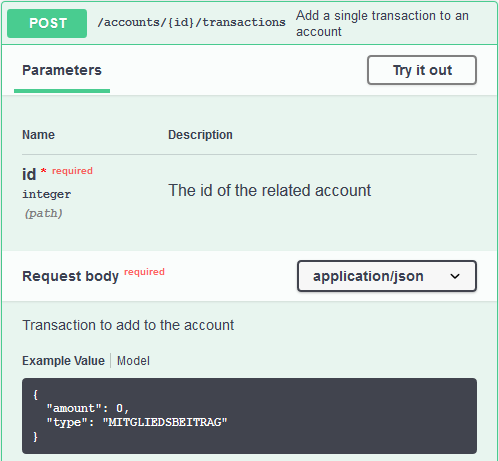
\includegraphics{images/api_spec_example_post.png}
    \caption{Notwendige Parameter für das Hinzufügen einer Transaktion zu einem
    Mitgliedskonto}
    \label{fig:api_spec_post}
\end{figure}

\section{Die Plattform}

% Github mit Repositories
Während die API-Spec die Schnittstelle zwischen Frontend und Backend
dokumentiert, wird der Quellcode auf der Plattform \emph{GitHub} verwaltet.
Frontend und Backend haben hier jeweils ein Repository des
Versionsverwaltungssystems \emph{Git}. Hier geschieht die Entwicklung
weitesgehend unabhängig, ausgenommen einiger Fälle in dem ein Mitglied des
einen Teams \emph{Issues} im Repository des anderen Teams eröffnet, um z.~B.
Bugs zu dokumentieren.

% Server als Integrationsumgebung
Um diese parallele Arbeit nun zusammenzuführen, also zu \emph{integrieren} und
um eine Instanz des aktuellen Entwicklungsstands der Applikation für den Kunden
oder die \emph{POs} zu haben, wird ein \emph{Integrationsserver} betrieben.
Auf diesem Server laufen das Frontend und das Backend.

%% Jenkins
Dabei wird die Integrations-Software \emph{Jenkins} benutzt. Jenkins prüft jede
Minute, ob es Änderungen auf dem Haupt- und Testzweig der Git-Repositories von
Frontend und Backend gibt. Wird eine Änderung gefunden, lädt Jenkins den
neuesten Quellcode, \emph{baut} eine lauffähige Anwendung \emph{kompilieren,
durchführen von Unit-Tests, verpacken zu bereitstellbaren Dateien} und liefert
diese dann an den jeweiligen Server. Dass Backend läuft auf einem
\emph{Tomcat}-Applikationsserver, dass Frontend wird von einem
\emph{nginx}-Webserver. Es laufen zwei Instanzen der App, \emph{Test} und \emph{Master}.

%% Der Pi
Für das fünfte Semester wurde als Server ein \emph{Raspberry Pi}-Bastelcomputer
mit Linux-Betriebssystem genutzt. Der \emph{Pi} hat einen relativ schwachen
Prozessor und kleinen Arbeitsspeicher, was dazu führte, dass es nicht möglich
war, dass Frontend auf dem \emph{Pi} zu bauen, da dieser dabei abstürzte. Es
wurde stattdessen das Frontend bereits gebaut \emph{händisch} bereitgestellt.

%% Die Büchse
Zu Beginn des sechsten Semesters wurde der von Prof. Dr. Engel bereitgestellte
Server in Betrieb genommen, der deutlich leistungsfähiger ist. Dadurch war es
nun auch möglich, dass Frontend komplett automatisiert bereitzustellen. 

\end{document}
